\chapter{Additional wall-resolved boundary layer profiles}
\label{app:zpg:wr-profiles}

This appendix supplements Section~\ref{sec:comparative:zpg:wall-resolved-baselines}
with the ten case comparisons accompanying the M6Tw025 and LowH\_M3 profiles
shown in the main text. The plots compare wall-resolved Spalart--Allmaras
and \(k\)--\(\omega\) SST predictions at \(Pr_t=0.9\) with the DNS references.
Matching conventions and reference-data limitations are described in
Section~\ref{sec:evaluation:benchmark-cases}.

\section{Martin--Duan Part 2}

The digitized profiles use the inferred temperature normalization described
in Section~\ref{sec:evaluation:benchmark-cases}. The published \(Re_{\delta2}\)
values remain nominal matching targets, subject to the inconsistency
discussed in Appendix~\ref{app:duan:reynolds}.

\begin{figure}[!htbp]
    \centering
    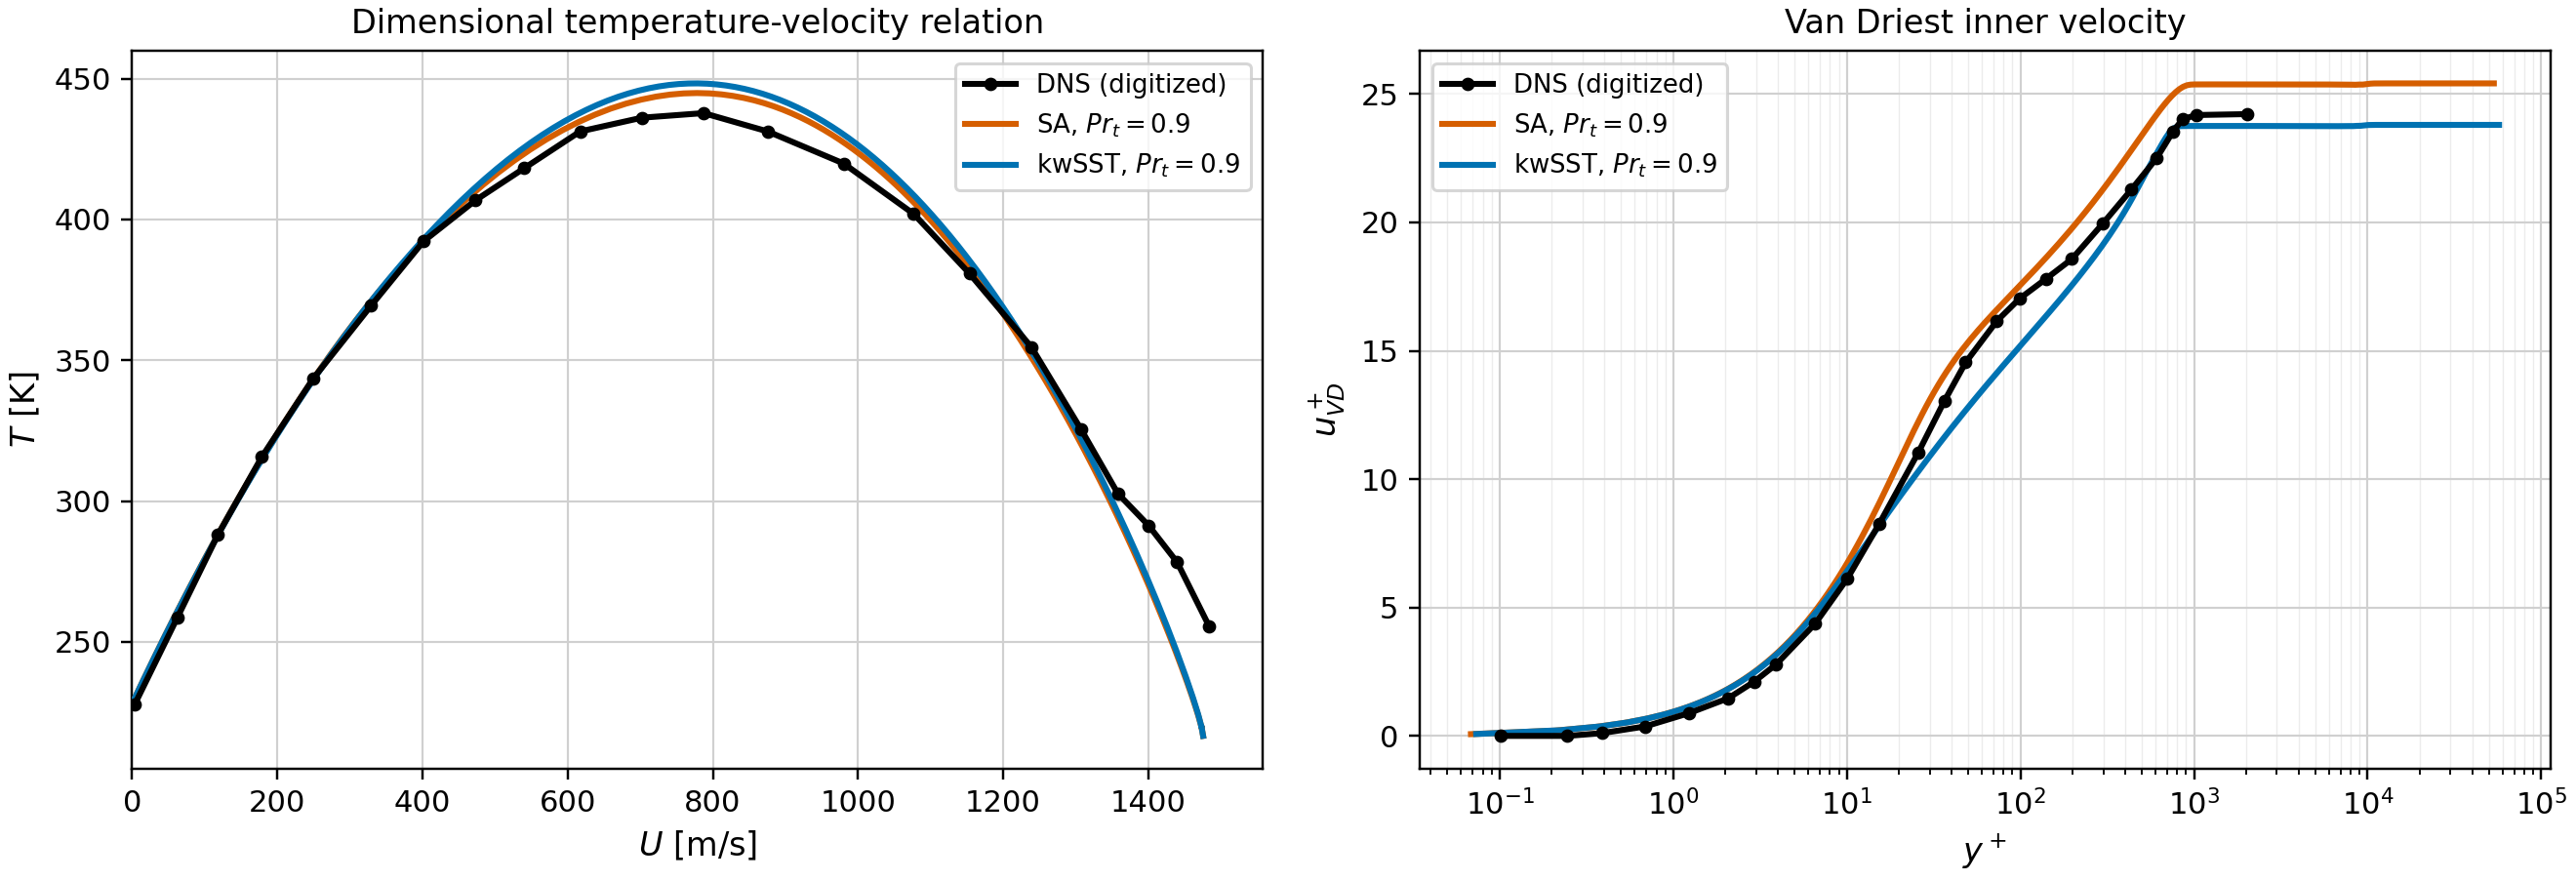
\includegraphics[width=\linewidth]{07_Error_Isolation_Results/Figures/Appendix/WR_BL_profile/Part2_M5T1_profiles.png}
    \caption[M5T1: wall-resolved boundary layer profiles]{Wall-resolved Spalart--Allmaras and \(k\)--\(\omega\) SST profiles for M5T1 at \(Pr_t=0.9\), compared with digitized Martin--Duan Part~2 DNS data~\cite{duan2010direct_part2}. Left: dimensional temperature--velocity relation \(T(U)\). Right: van Driest--transformed velocity \(U_{\mathrm{VD}}^+\) versus wall distance \(y^+\) at the matched \(Re_{\delta2}\) = 1538.4 station.}
    \label{fig:app:zpg:profiles:M5T1}
\end{figure}

\begin{figure}[!htbp]
    \centering
    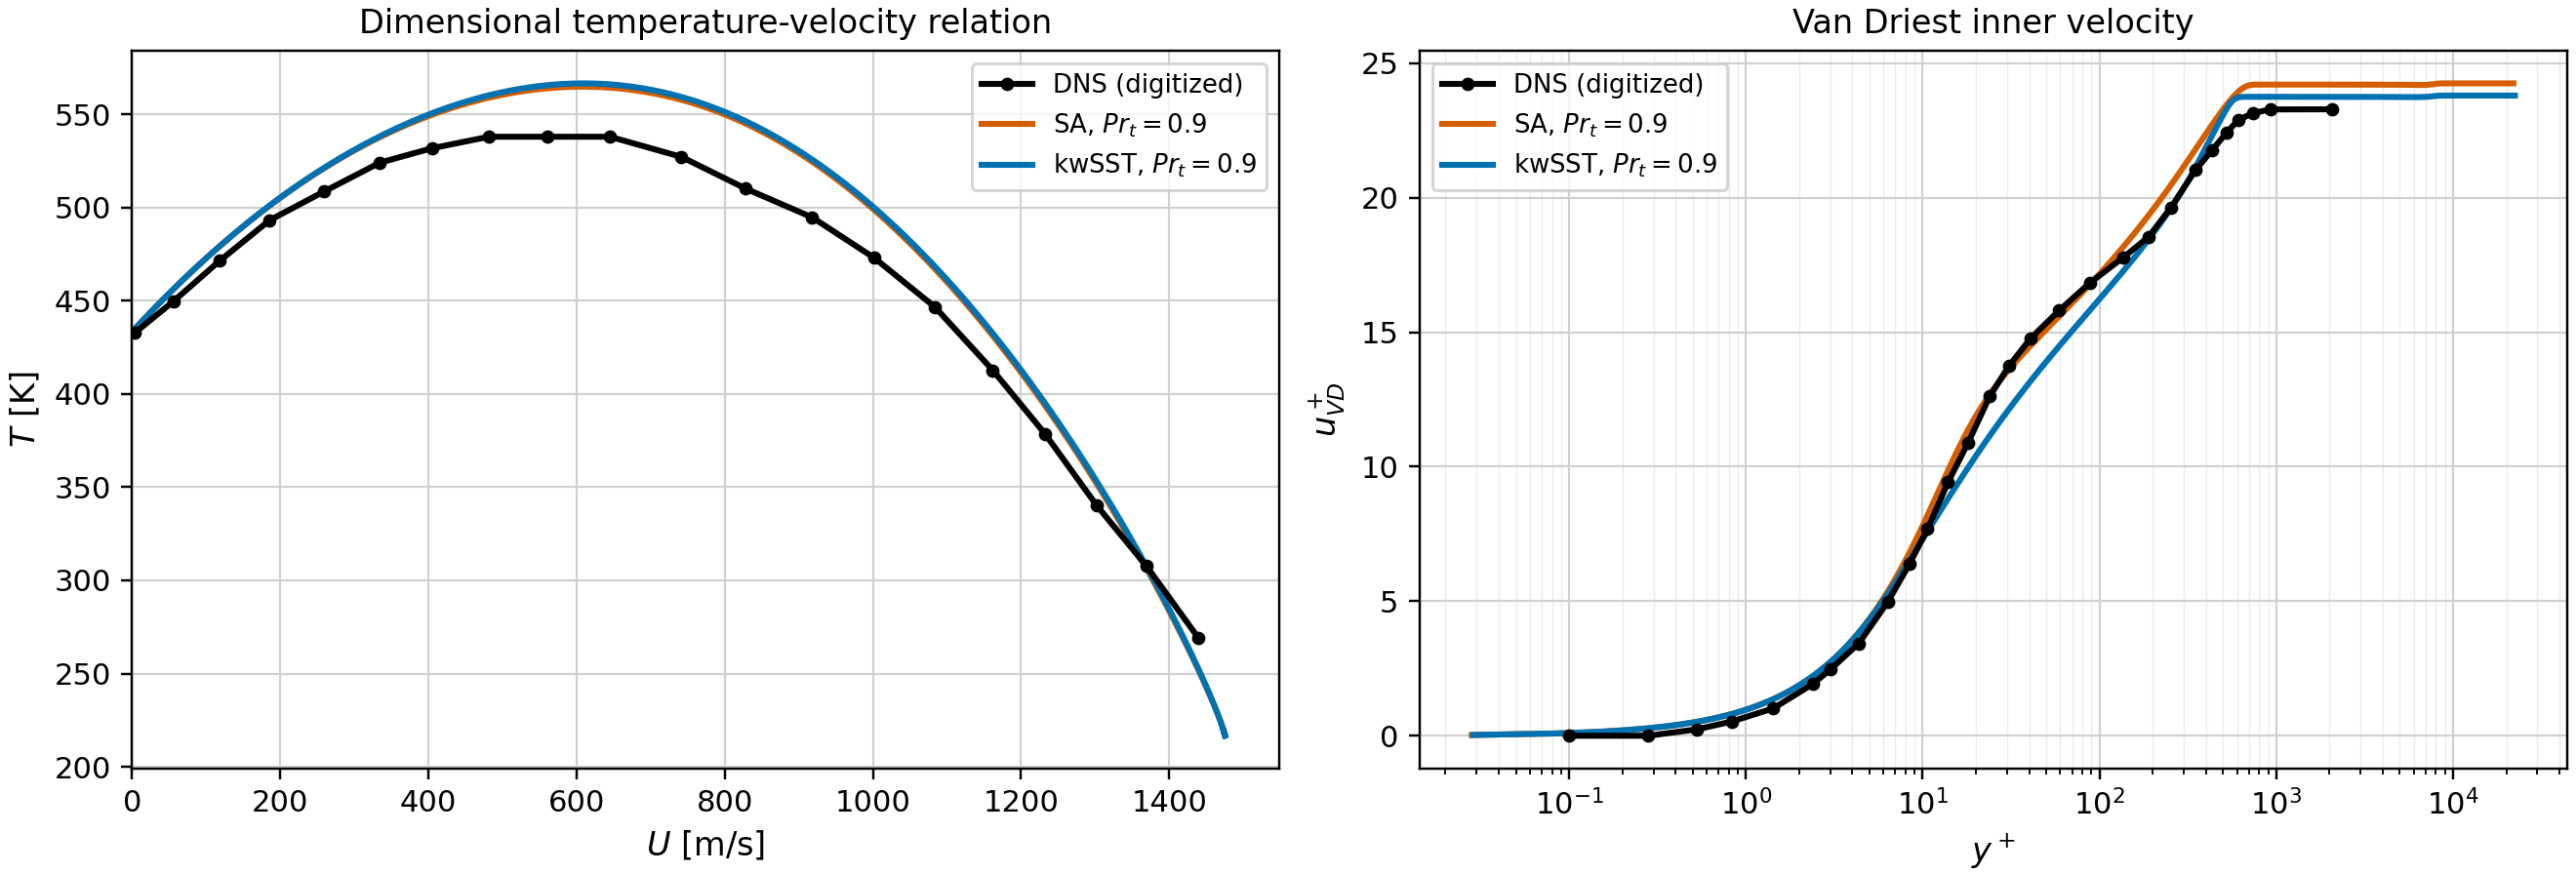
\includegraphics[width=\linewidth]{07_Error_Isolation_Results/Figures/Appendix/WR_BL_profile/Part2_M5T2_profiles.png}
    \caption[M5T2: wall-resolved boundary layer profiles]{Wall-resolved Spalart--Allmaras and \(k\)--\(\omega\) SST profiles for M5T2 at \(Pr_t=0.9\), compared with digitized Martin--Duan Part~2 DNS data~\cite{duan2010direct_part2}. Left: dimensional temperature--velocity relation \(T(U)\). Right: van Driest--transformed velocity \(U_{\mathrm{VD}}^+\) versus wall distance \(y^+\) at the matched \(Re_{\delta2}\) = 1521.5 station.}
    \label{fig:app:zpg:profiles:M5T2}
\end{figure}

\begin{figure}[!htbp]
    \centering
    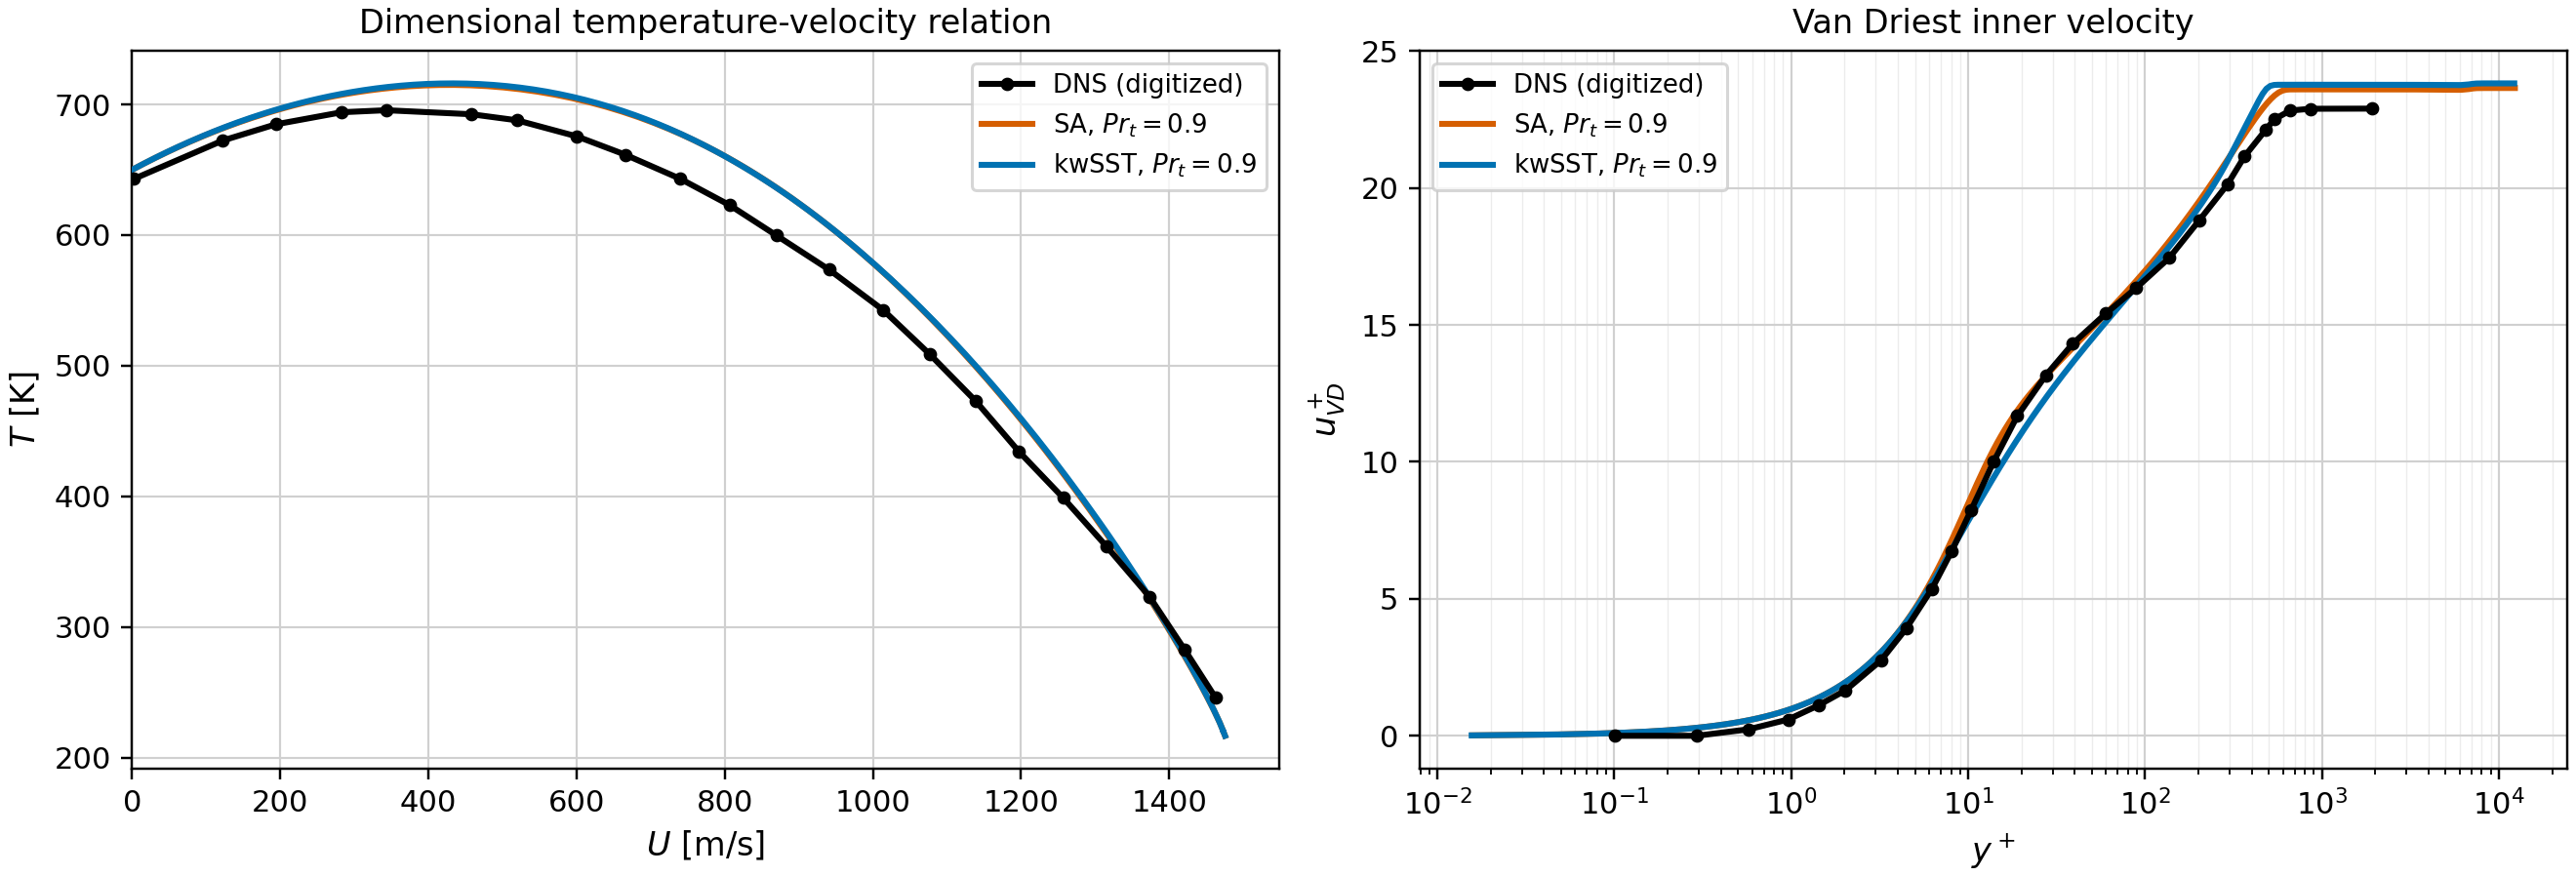
\includegraphics[width=\linewidth]{07_Error_Isolation_Results/Figures/Appendix/WR_BL_profile/Part2_M5T3_profiles.png}
    \caption[M5T3: wall-resolved boundary layer profiles]{Wall-resolved Spalart--Allmaras and \(k\)--\(\omega\) SST profiles for M5T3 at \(Pr_t=0.9\), compared with digitized Martin--Duan Part~2 DNS data~\cite{duan2010direct_part2}. Left: dimensional temperature--velocity relation \(T(U)\). Right: van Driest--transformed velocity \(U_{\mathrm{VD}}^+\) versus wall distance \(y^+\) at the matched \(Re_{\delta2}\) = 1524.7 station.}
    \label{fig:app:zpg:profiles:M5T3}
\end{figure}

\begin{figure}[!htbp]
    \centering
    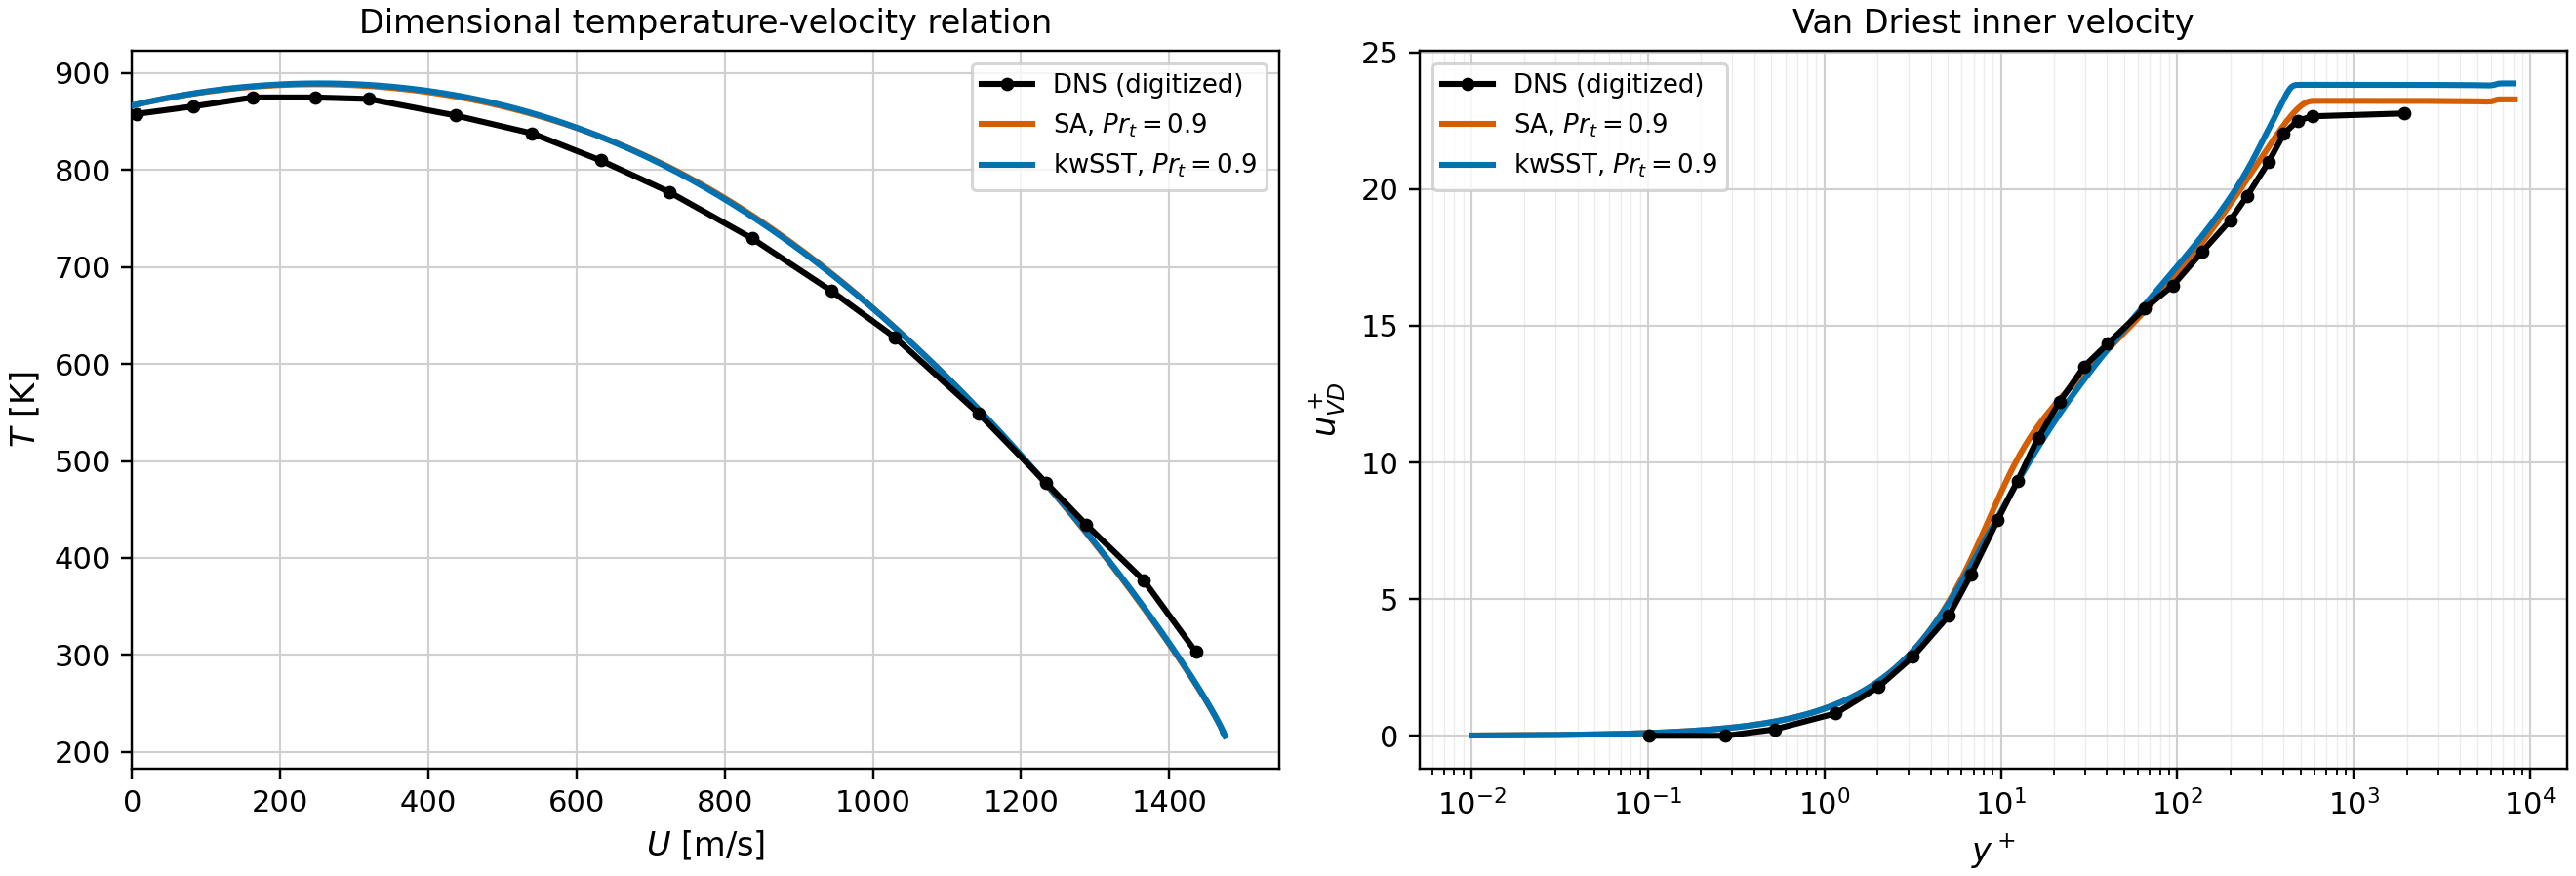
\includegraphics[width=\linewidth]{07_Error_Isolation_Results/Figures/Appendix/WR_BL_profile/Part2_M5T4_profiles.png}
    \caption[M5T4: wall-resolved boundary layer profiles]{Wall-resolved Spalart--Allmaras and \(k\)--\(\omega\) SST profiles for M5T4 at \(Pr_t=0.9\), compared with digitized Martin--Duan Part~2 DNS data~\cite{duan2010direct_part2}. Left: dimensional temperature--velocity relation \(T(U)\). Right: van Driest--transformed velocity \(U_{\mathrm{VD}}^+\) versus wall distance \(y^+\) at the matched \(Re_{\delta2}\) = 1526.4 station.}
    \label{fig:app:zpg:profiles:M5T4}
\end{figure}

\begin{figure}[!htbp]
    \centering
    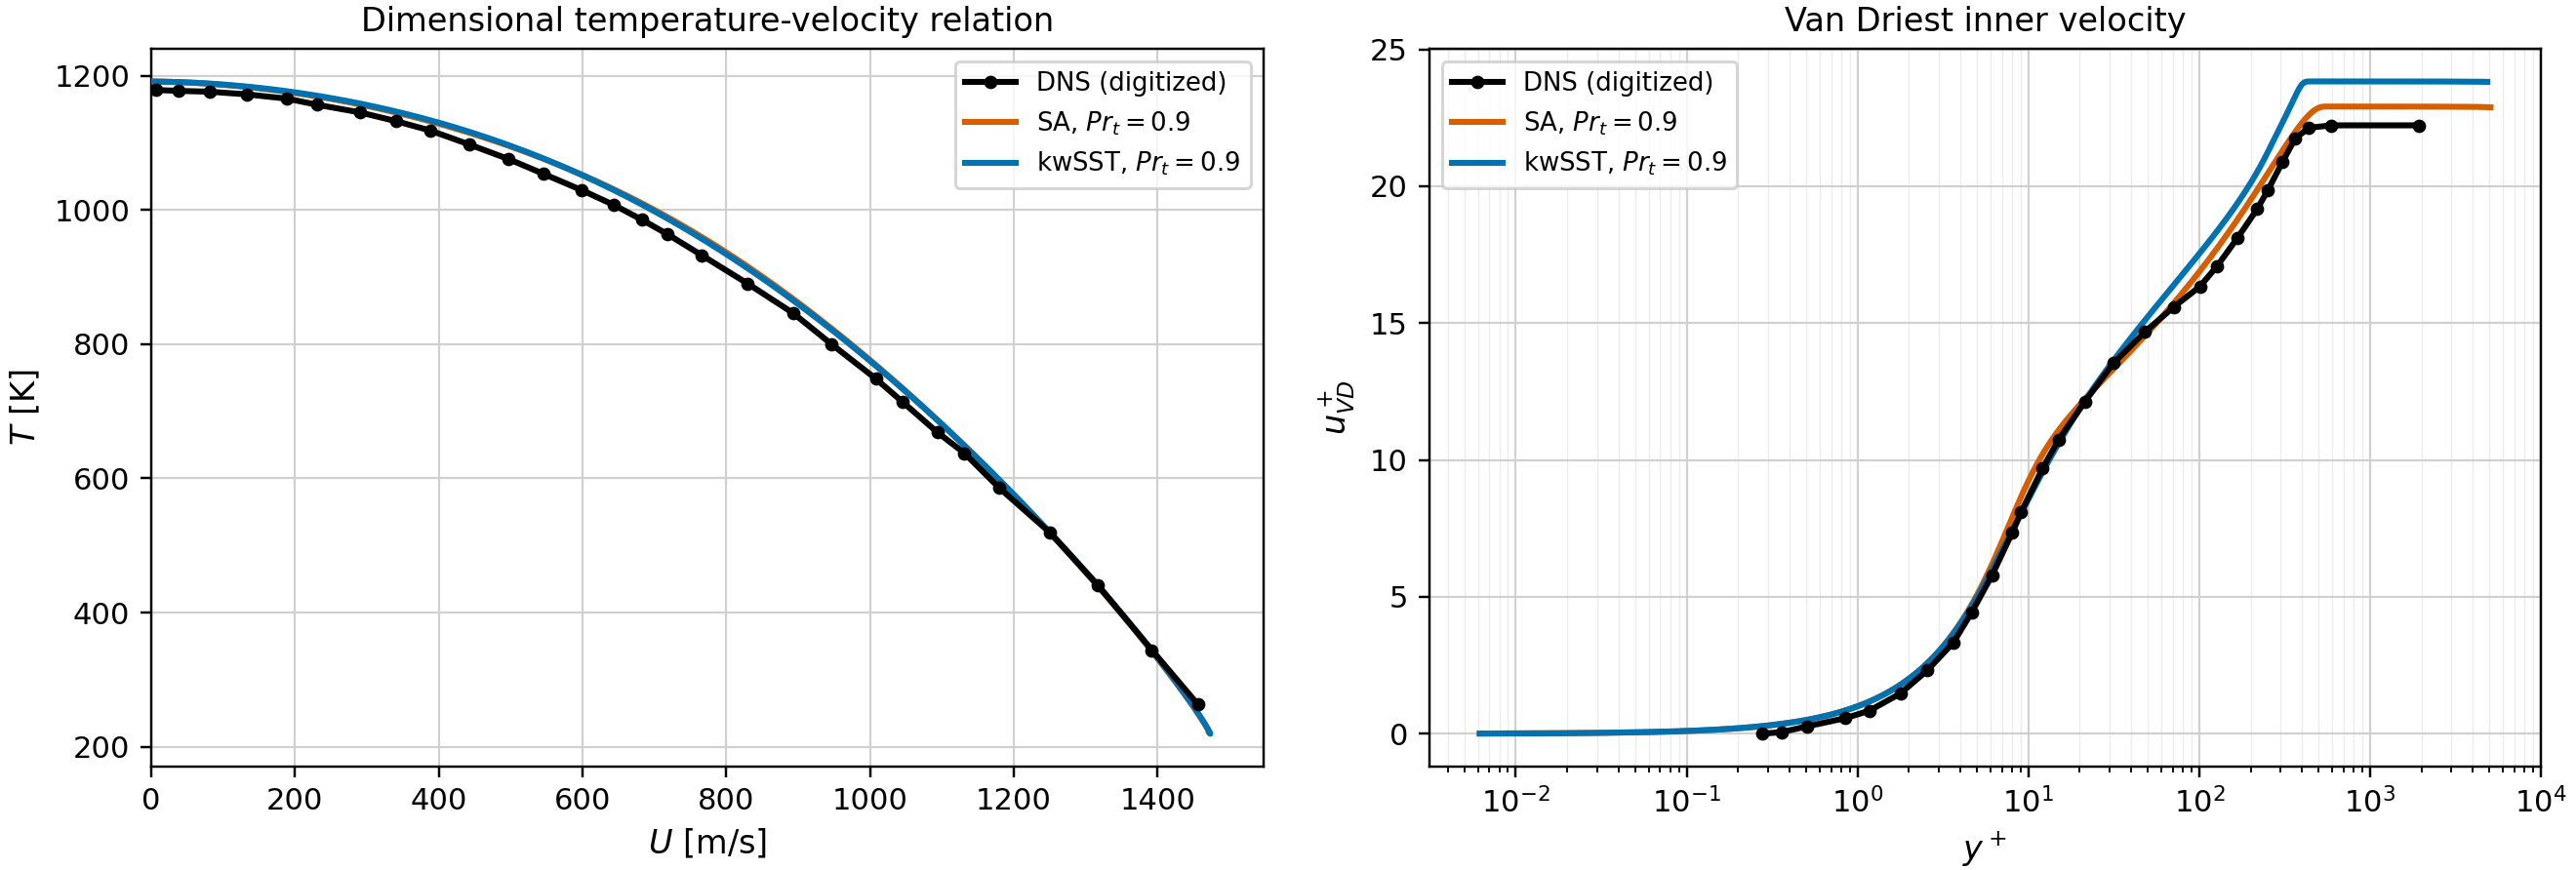
\includegraphics[width=\linewidth]{07_Error_Isolation_Results/Figures/Appendix/WR_BL_profile/Part2_M5T5_profiles.png}
    \caption[M5T5: wall-resolved boundary layer profiles]{Wall-resolved Spalart--Allmaras and \(k\)--\(\omega\) SST profiles for M5T5 at \(Pr_t=0.9\), compared with digitized Martin--Duan Part~2 DNS data~\cite{duan2010direct_part2}. Left: dimensional temperature--velocity relation \(T(U)\). Right: van Driest--transformed velocity \(U_{\mathrm{VD}}^+\) versus wall distance \(y^+\) at the matched \(Re_{\delta2}\) = 1536.8 station.}
    \label{fig:app:zpg:profiles:M5T5}
\end{figure}

\clearpage
\section{Zhang cases}

The following comparisons use the digital DNS profiles of
Zhang et al.~\cite{zhang2018direct}. The M6Tw076 profiles are retained as
qualitative comparisons; the wall-temperature inconsistency and limitations
on quantitative heat-flux assessment remain those described in
Section~\ref{sec:evaluation:benchmark-cases}.

\begin{figure}[!htbp]
    \centering
    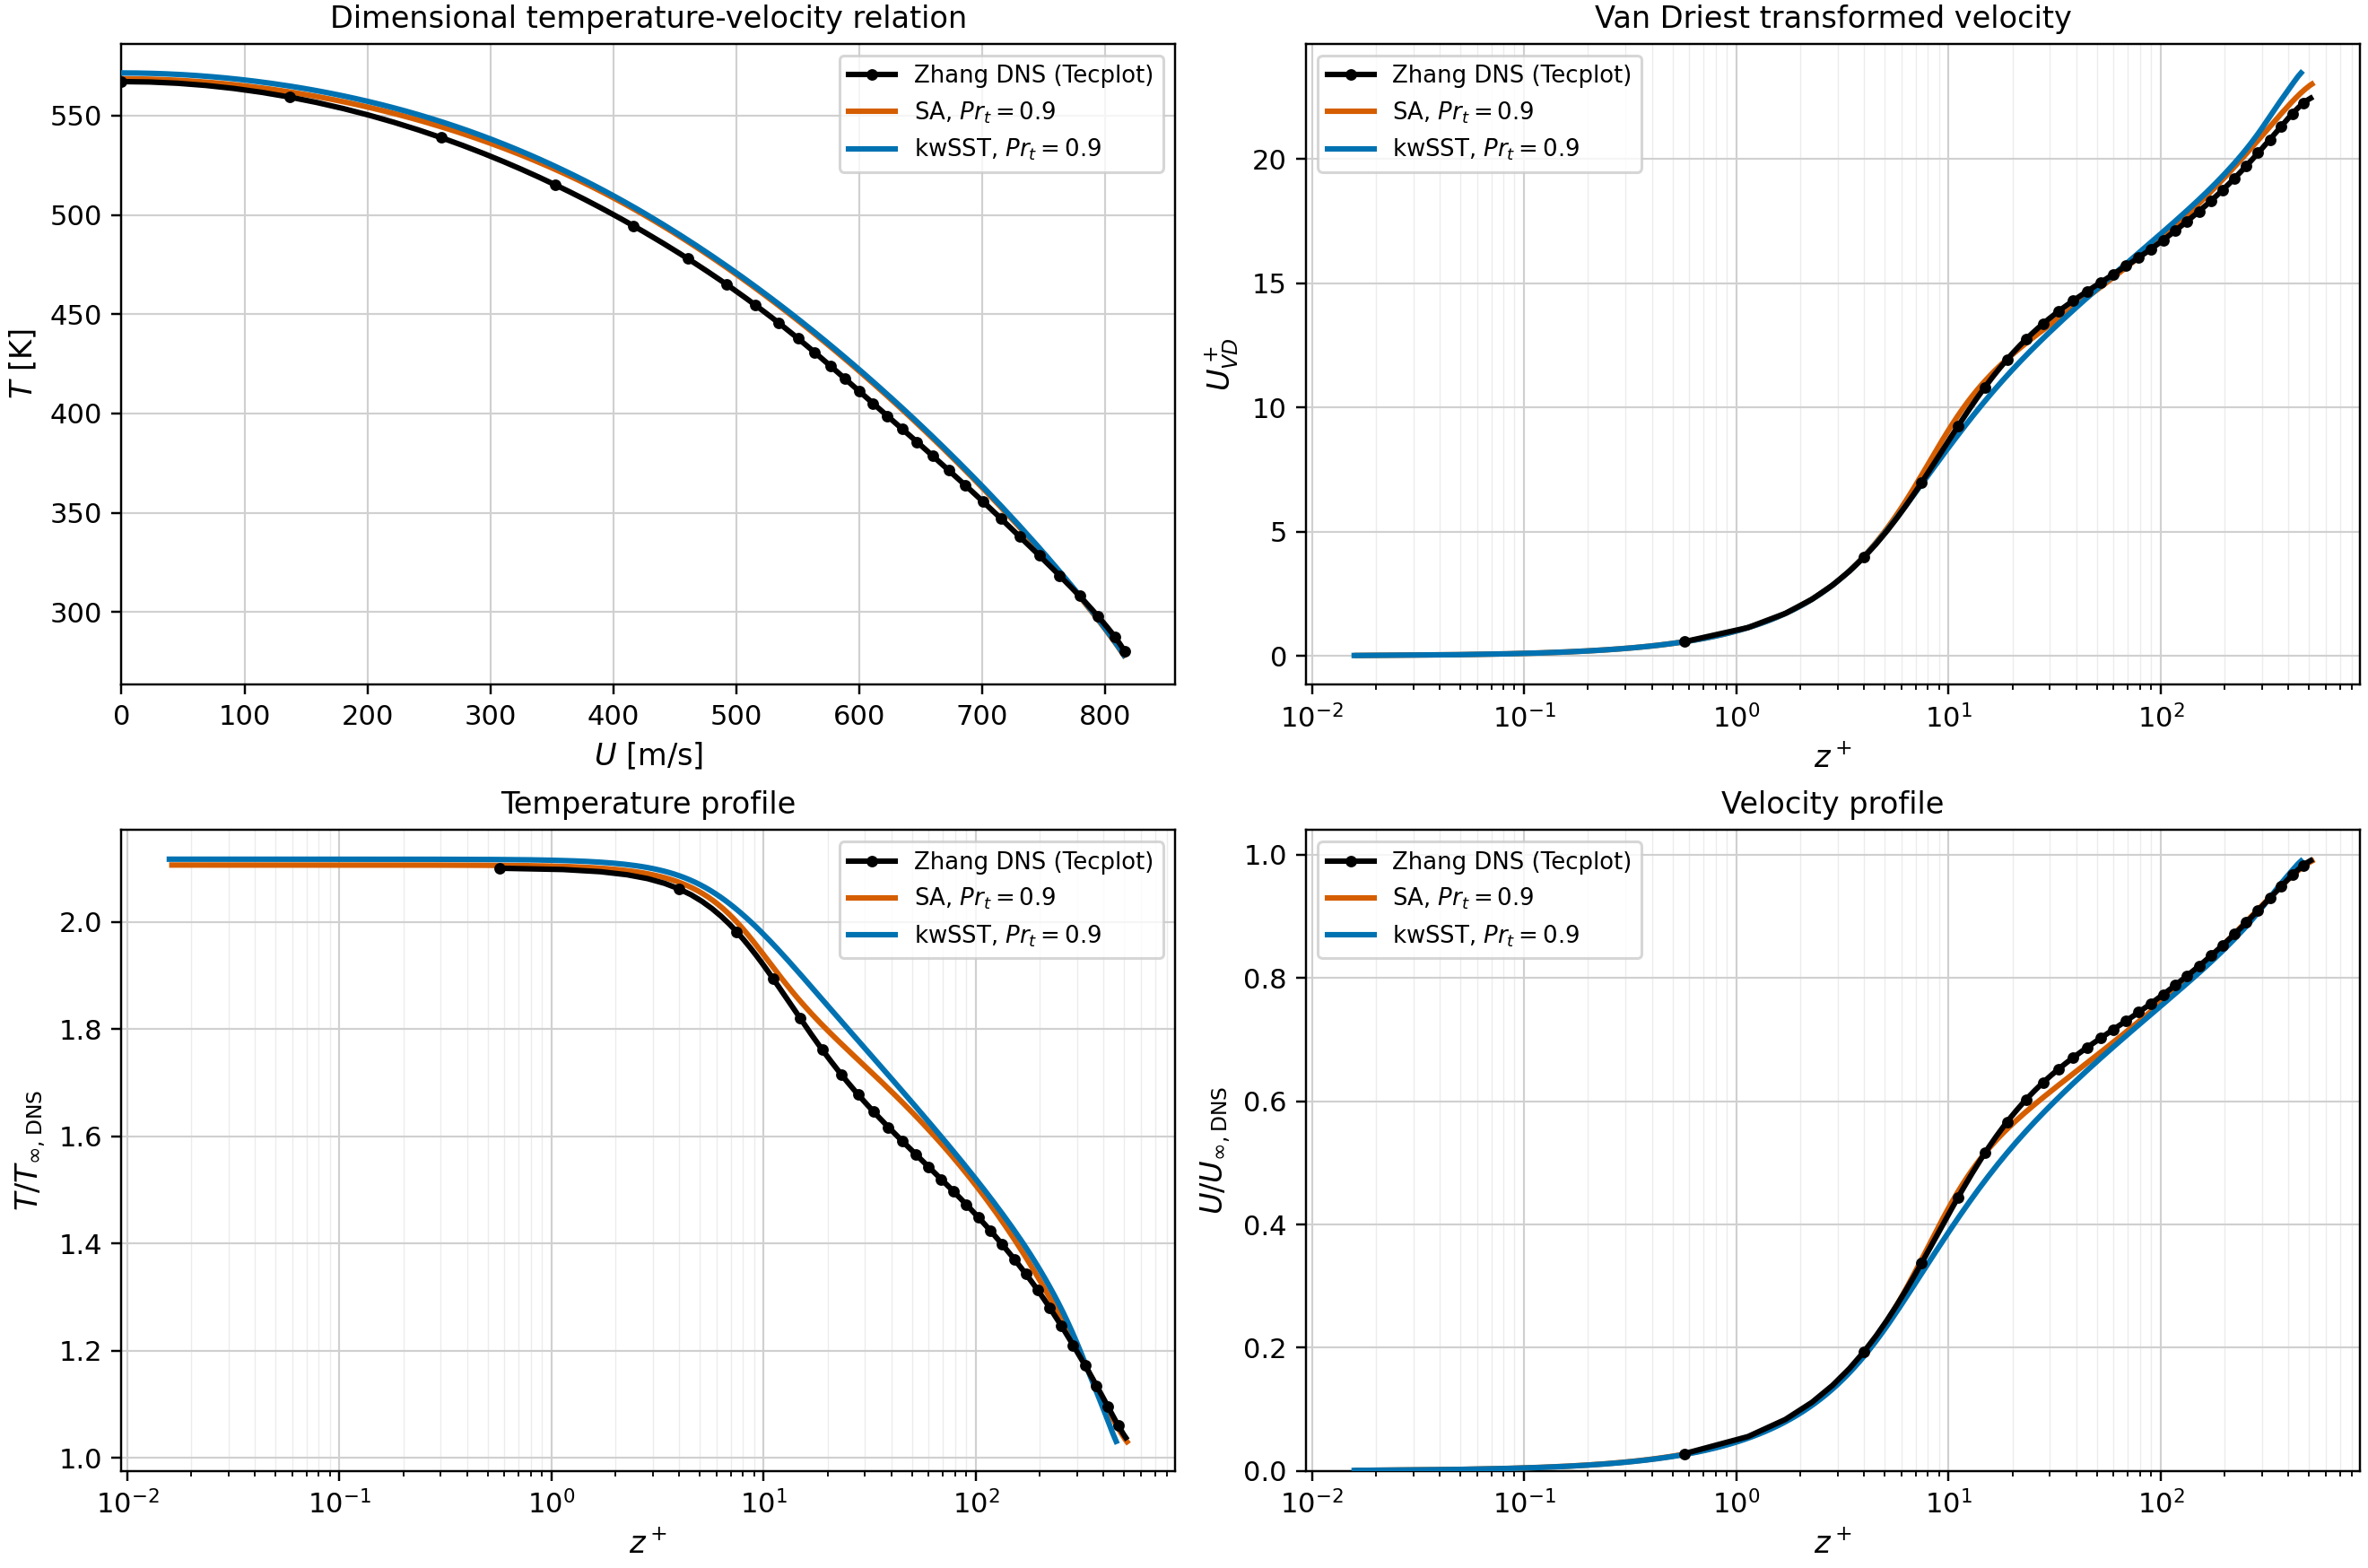
\includegraphics[width=\linewidth]{07_Error_Isolation_Results/Figures/Appendix/WR_BL_profile/M2p5_profiles.png}
    \caption[M2p5: wall-resolved boundary layer profiles]{Wall-resolved Spalart--Allmaras and \(k\)--\(\omega\) SST profiles for M2p5 at \(Pr_t=0.9\), compared with Zhang et al.'s DNS~\cite{zhang2018direct}. Top: dimensional \(T(U)\) (left) and van Driest--transformed velocity \(U_{\mathrm{VD}}^+\) versus \(z^+\) (right). Bottom: \(T/T_{\infty,\mathrm{DNS}}\) (left) and \(U/U_{\infty,\mathrm{DNS}}\) (right), both versus \(z^+\) at the matched \(Re_{\delta2}\) = 1657 station.}
    \label{fig:app:zpg:profiles:M2p5}
\end{figure}

\clearpage

\begin{figure}[!htbp]
    \centering
    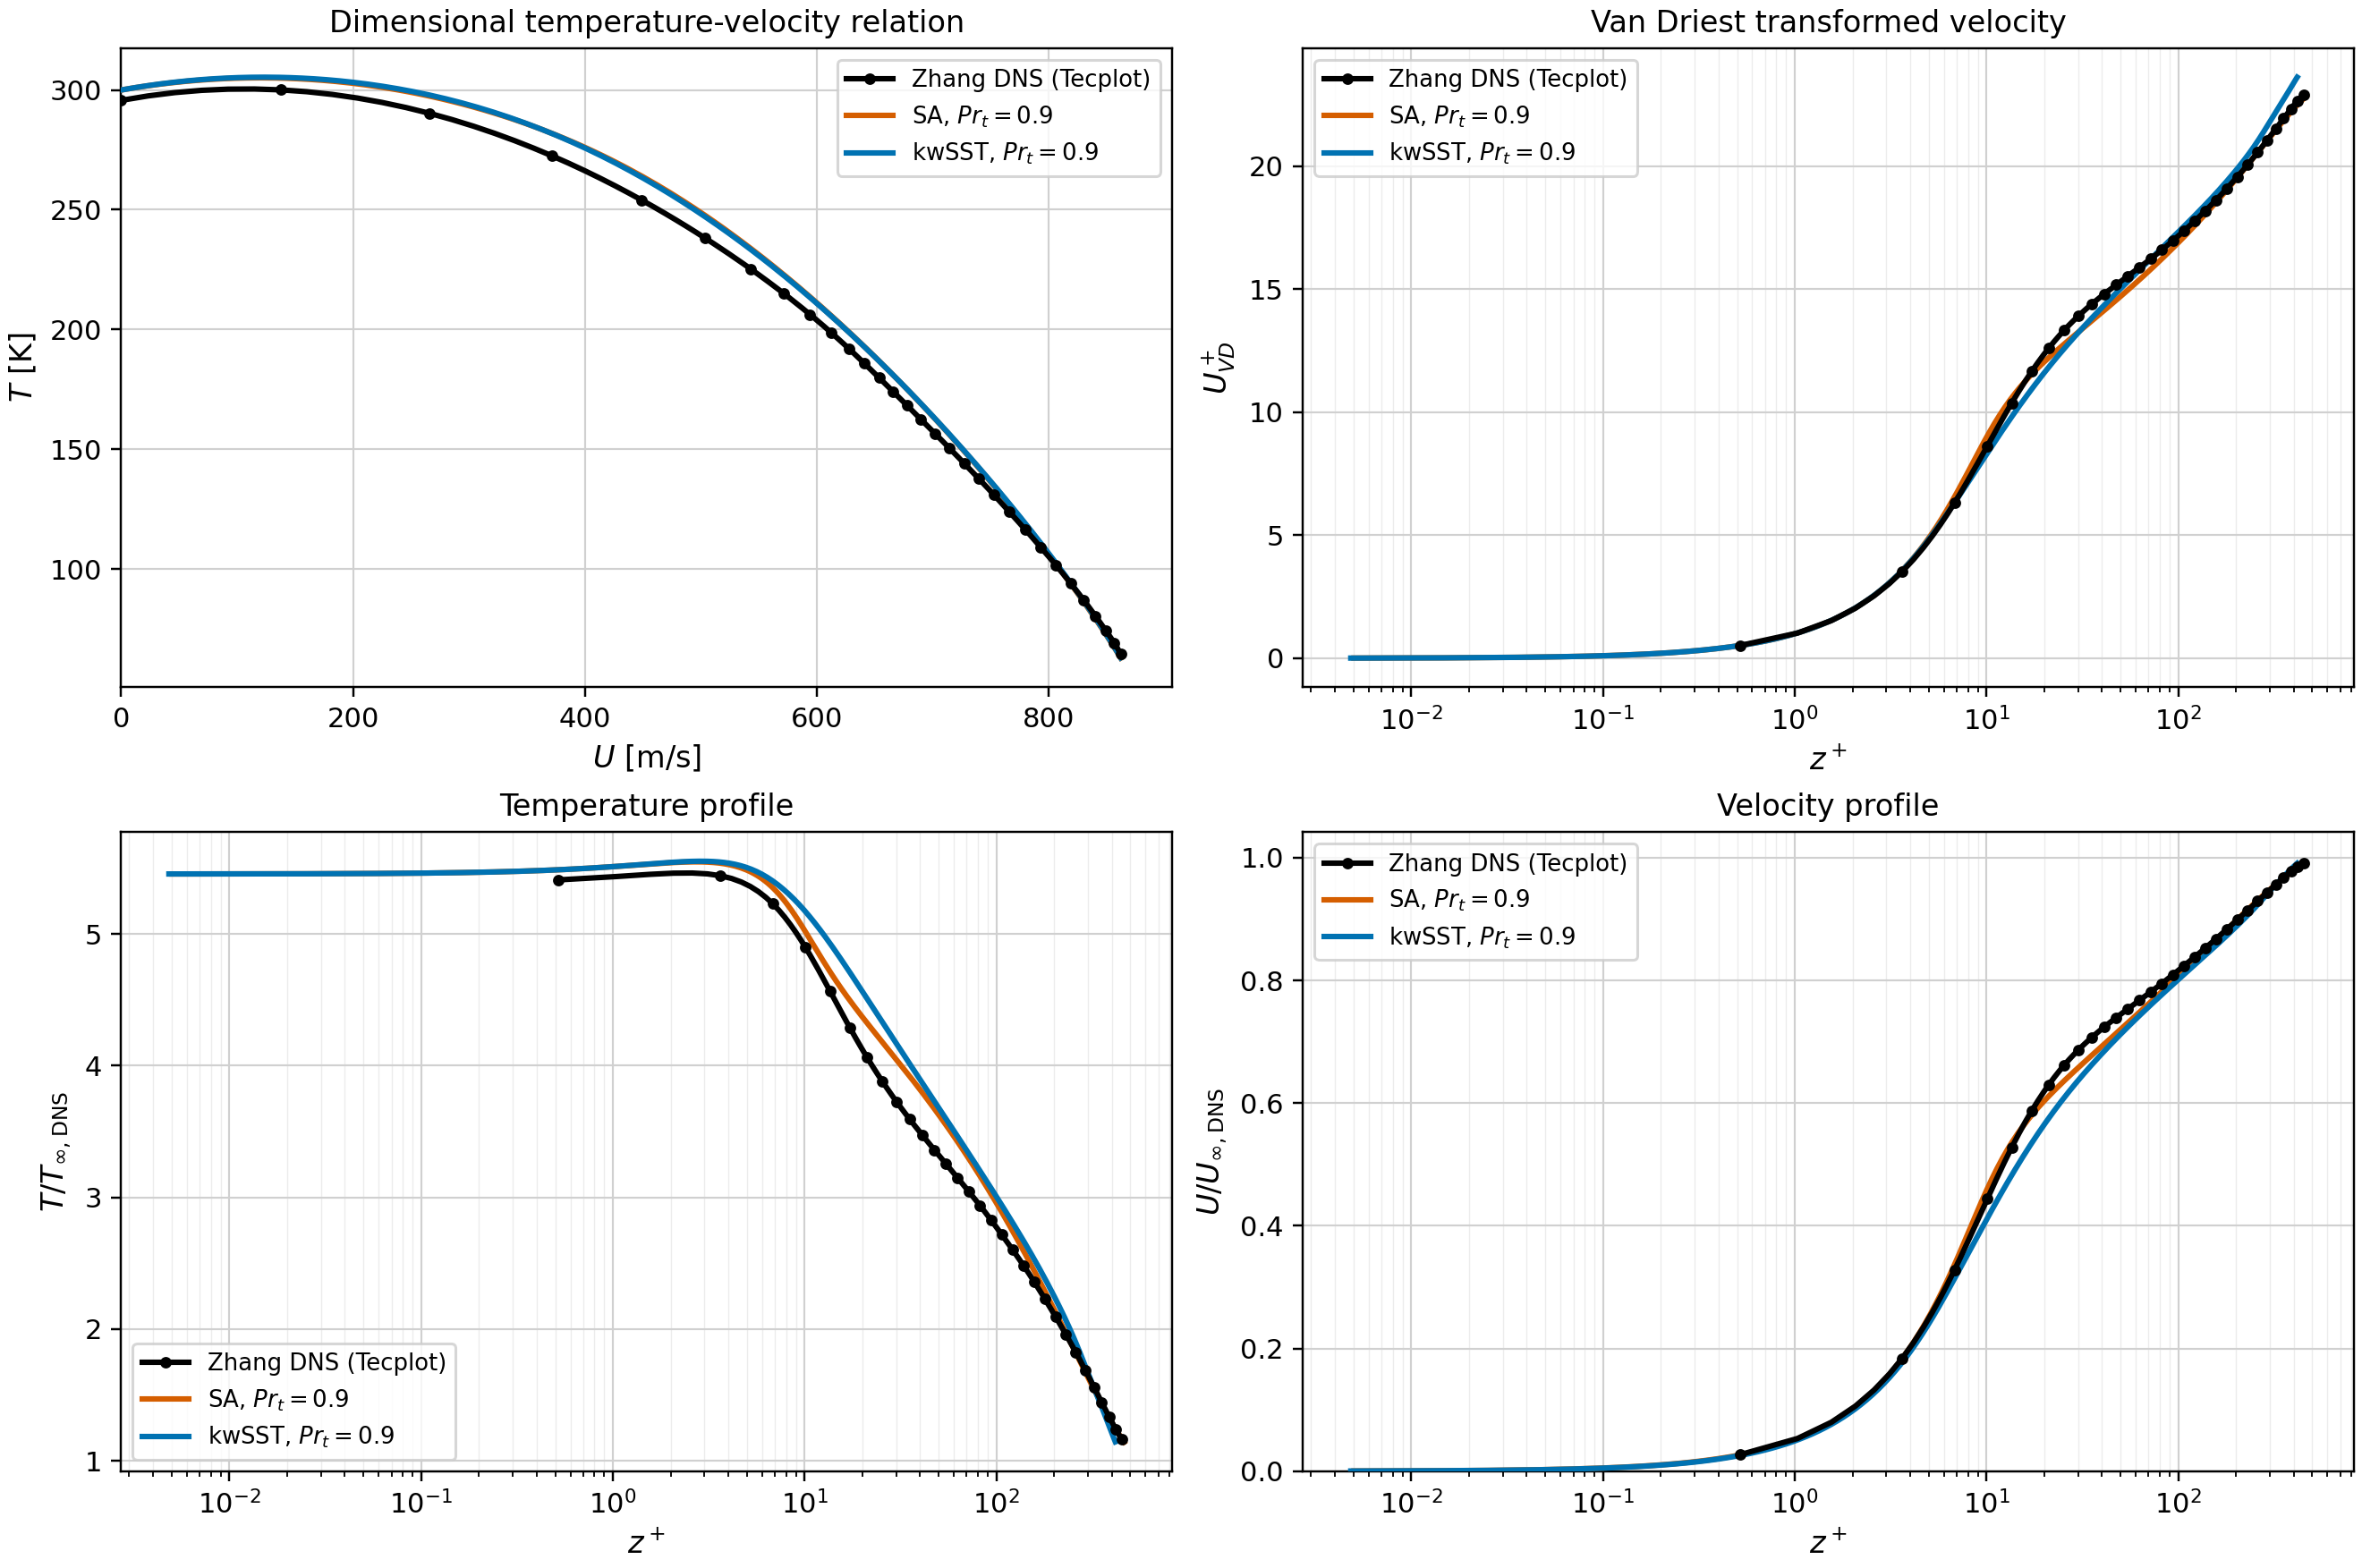
\includegraphics[width=\linewidth]{07_Error_Isolation_Results/Figures/Appendix/WR_BL_profile/M6Tw076_profiles.png}
    \caption[M6Tw076: wall-resolved boundary layer profiles]{Wall-resolved Spalart--Allmaras and \(k\)--\(\omega\) SST profiles for M6Tw076 at \(Pr_t=0.9\), compared with Zhang et al.'s DNS~\cite{zhang2018direct}. Top: dimensional \(T(U)\) (left) and van Driest--transformed velocity \(U_{\mathrm{VD}}^+\) versus \(z^+\) (right). Bottom: \(T/T_{\infty,\mathrm{DNS}}\) (left) and \(U/U_{\infty,\mathrm{DNS}}\) (right), both versus \(z^+\) at the matched \(Re_{\delta2}\) = 1746 station.}
    \label{fig:app:zpg:profiles:M6Tw076}
\end{figure}

\clearpage

\begin{figure}[!htbp]
    \centering
    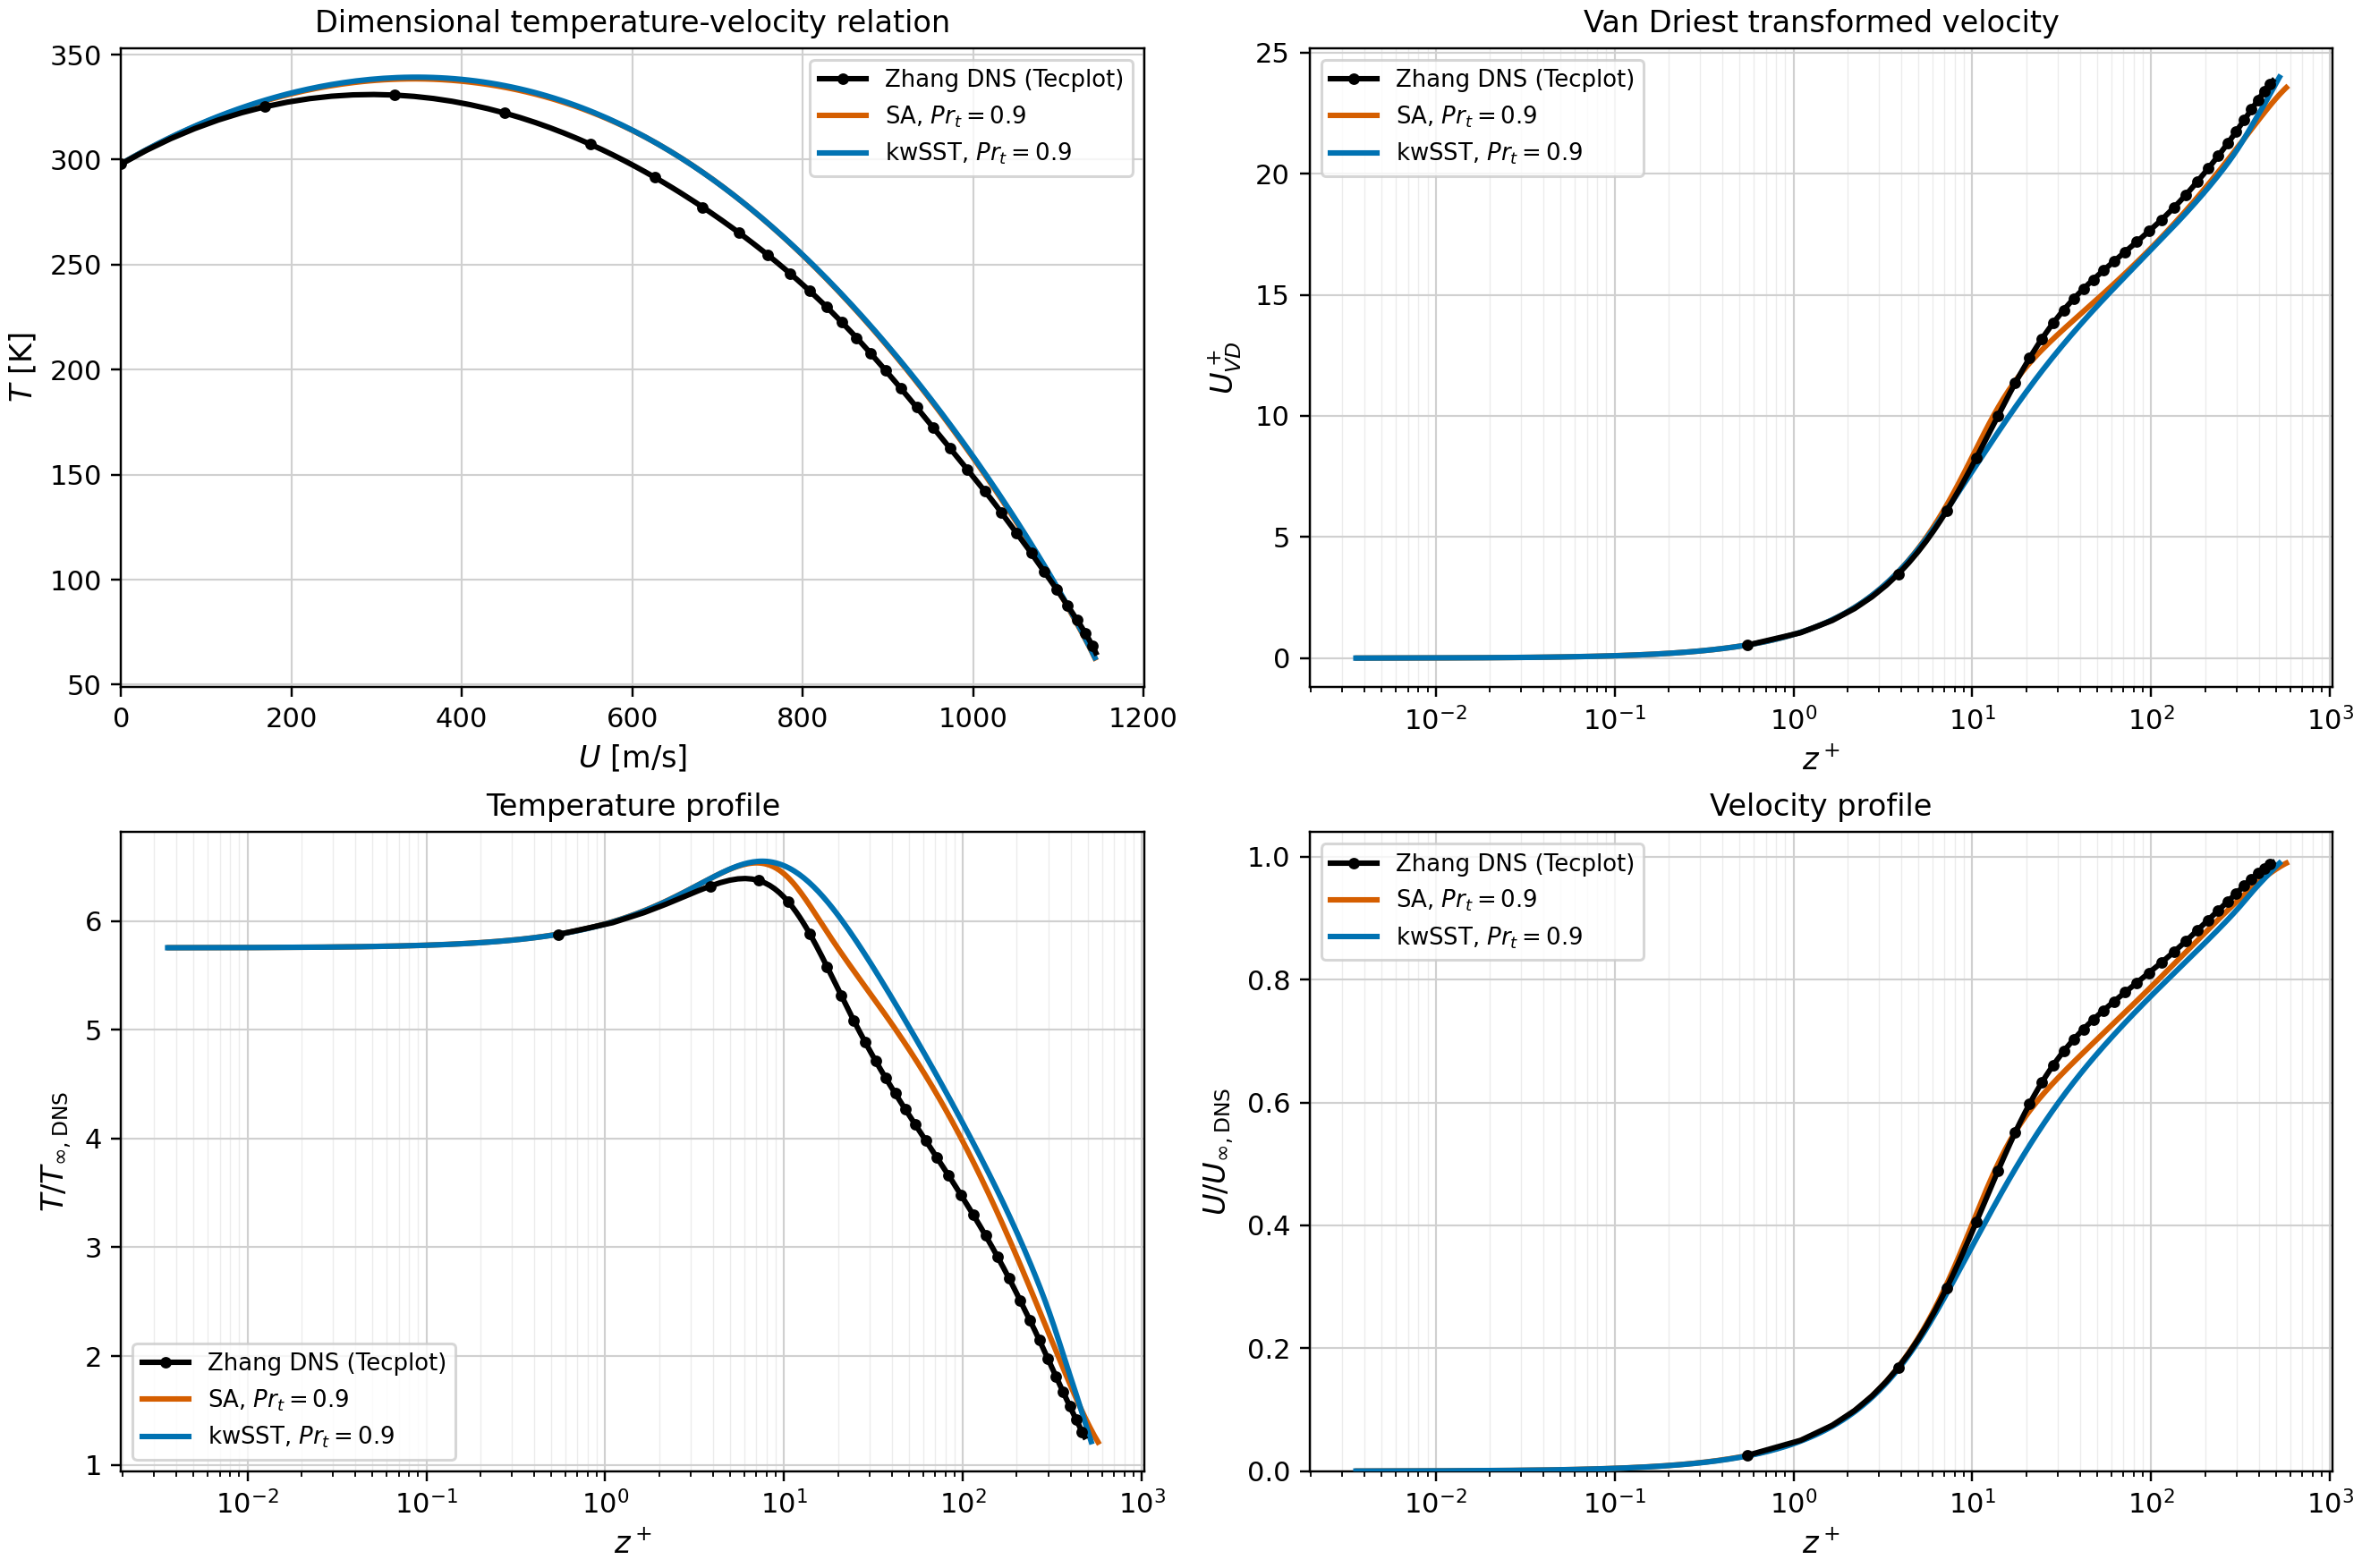
\includegraphics[width=\linewidth]{07_Error_Isolation_Results/Figures/Appendix/WR_BL_profile/M8Tw048_profiles.png}
    \caption[M8Tw048: wall-resolved boundary layer profiles]{Wall-resolved Spalart--Allmaras and \(k\)--\(\omega\) SST profiles for M8Tw048 at \(Pr_t=0.9\), compared with Zhang et al.'s DNS~\cite{zhang2018direct}. Top: dimensional \(T(U)\) (left) and van Driest--transformed velocity \(U_{\mathrm{VD}}^+\) versus \(z^+\) (right). Bottom: \(T/T_{\infty,\mathrm{DNS}}\) (left) and \(U/U_{\infty,\mathrm{DNS}}\) (right), both versus \(z^+\) at the matched \(Re_{\delta2}\) = 1990 station.}
    \label{fig:app:zpg:profiles:M8Tw048}
\end{figure}

\clearpage

\begin{figure}[!htbp]
    \centering
    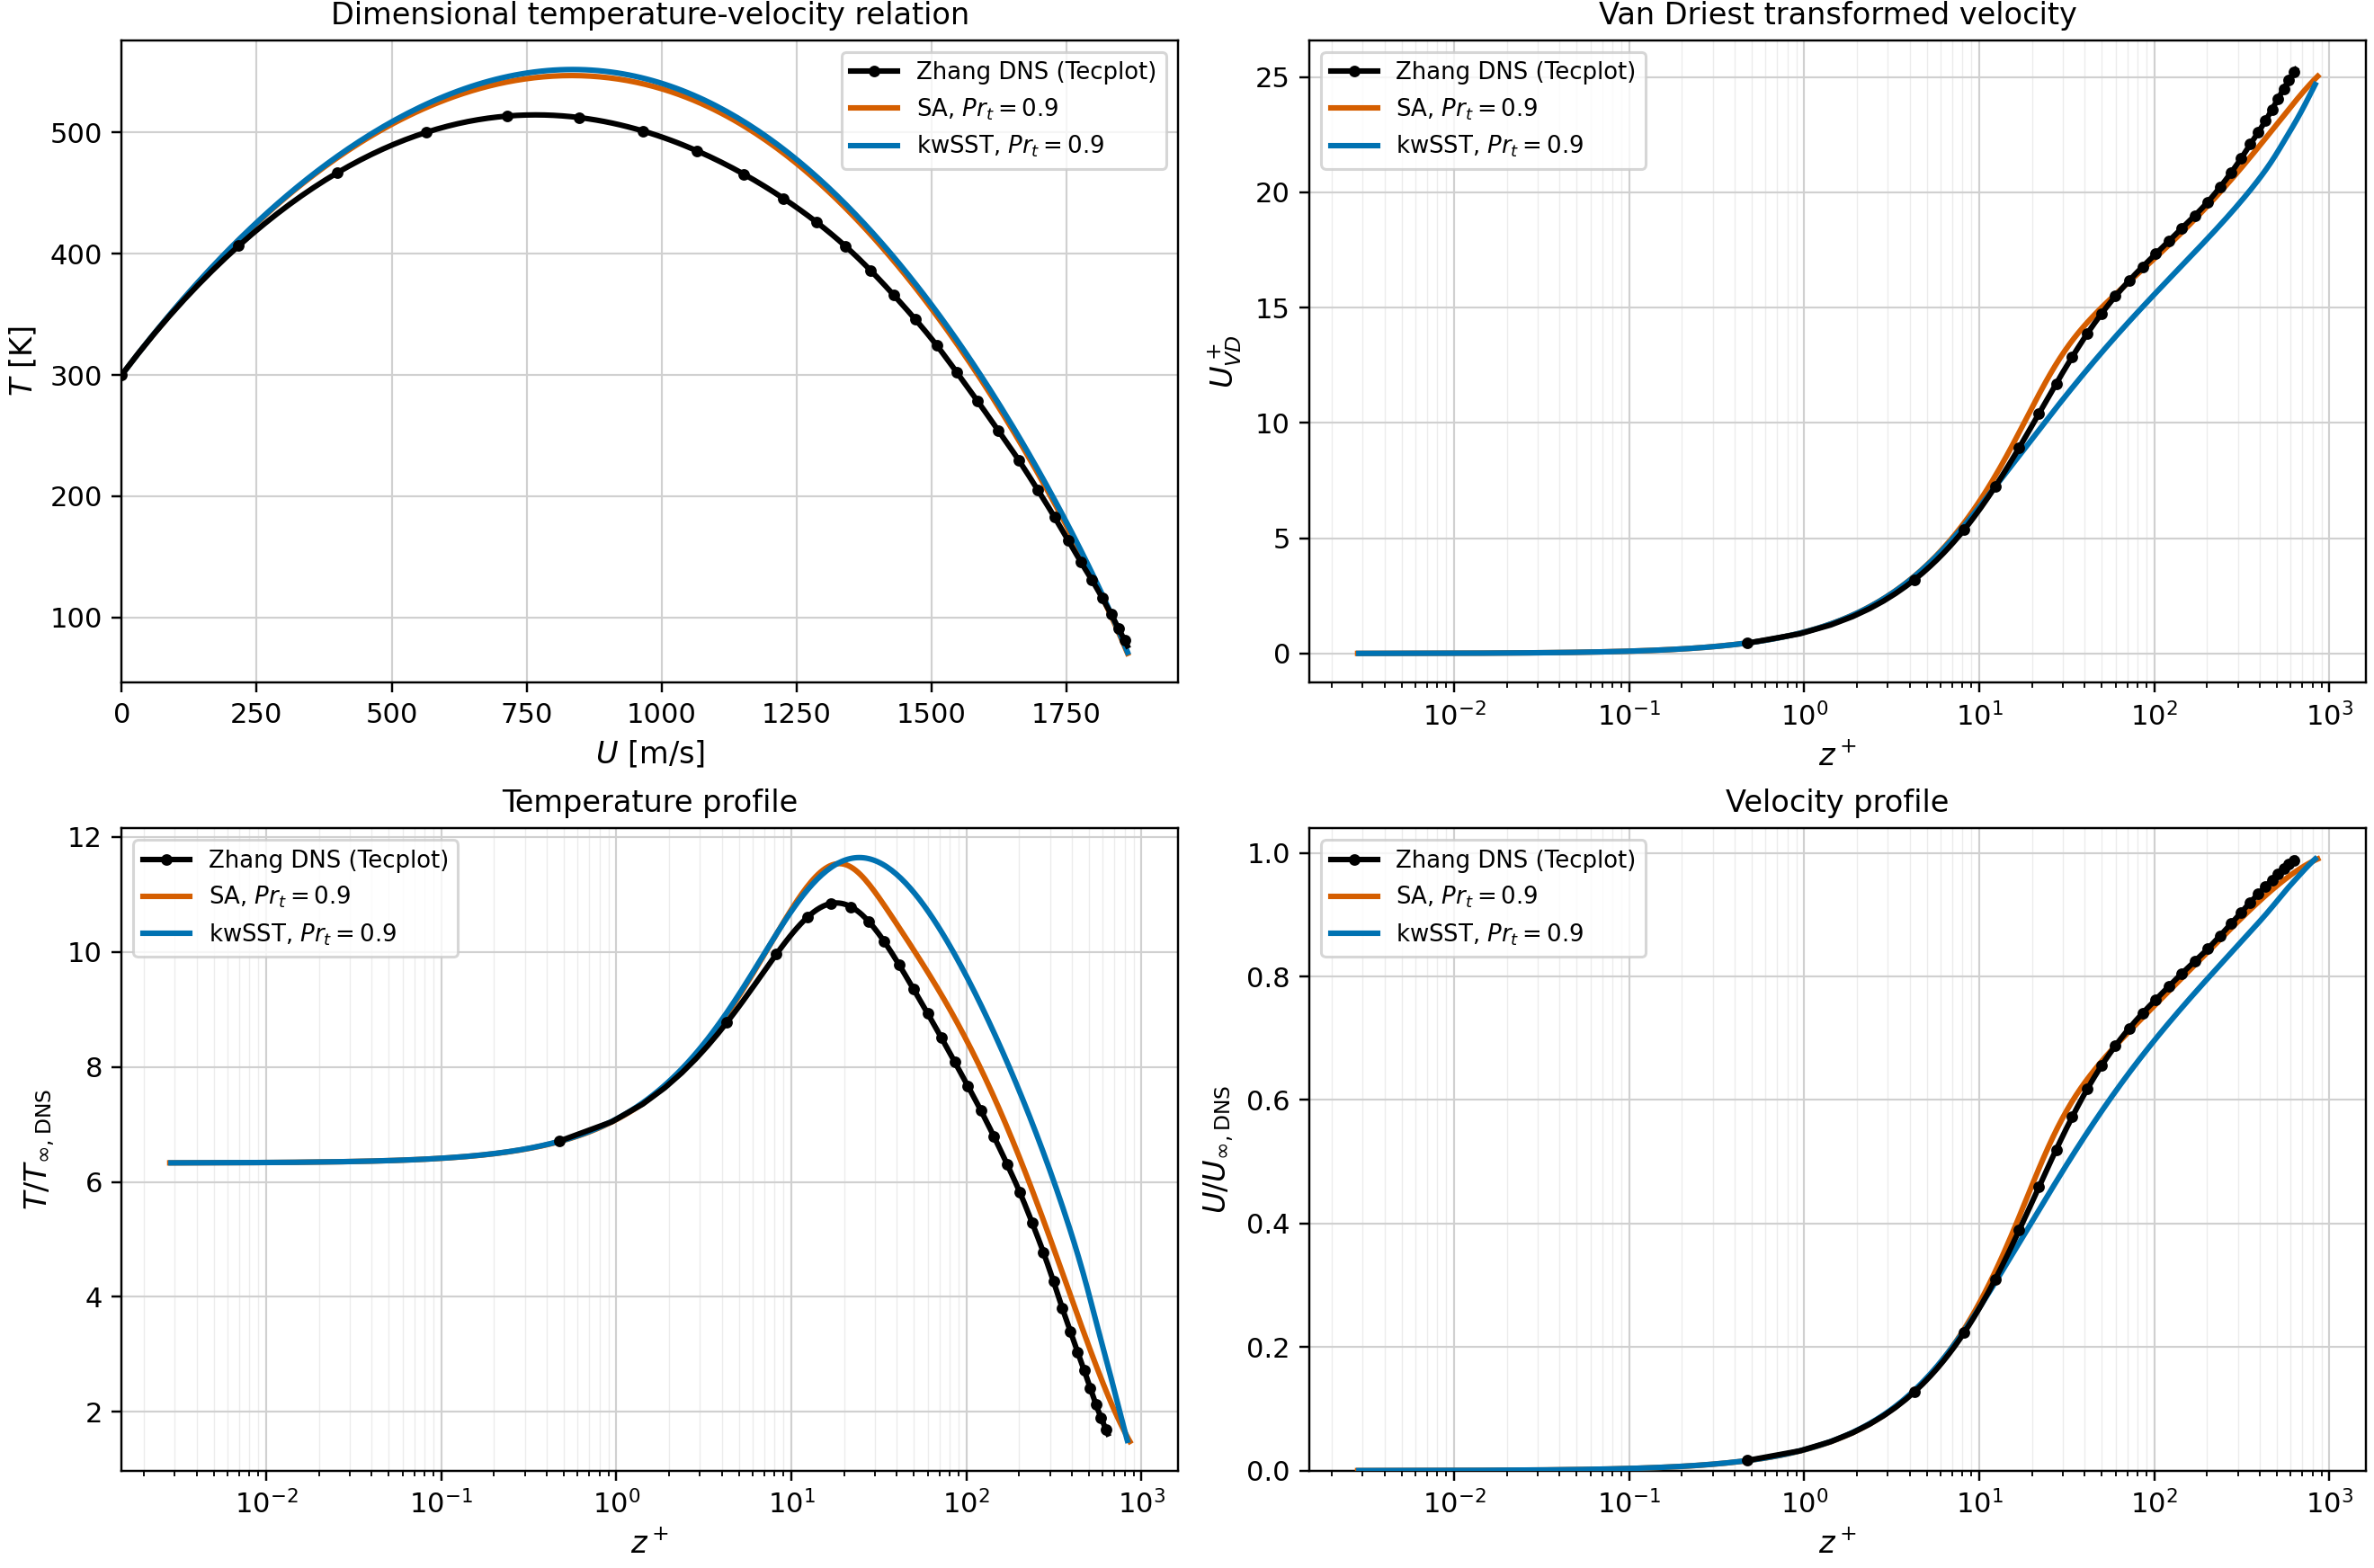
\includegraphics[width=\linewidth]{07_Error_Isolation_Results/Figures/Appendix/WR_BL_profile/M14Tw018_profiles.png}
    \caption[M14Tw018: wall-resolved boundary layer profiles]{Wall-resolved Spalart--Allmaras and \(k\)--\(\omega\) SST profiles for M14Tw018 at \(Pr_t=0.9\), compared with Zhang et al.'s DNS~\cite{zhang2018direct}. Top: dimensional \(T(U)\) (left) and van Driest--transformed velocity \(U_{\mathrm{VD}}^+\) versus \(z^+\) (right). Bottom: \(T/T_{\infty,\mathrm{DNS}}\) (left) and \(U/U_{\infty,\mathrm{DNS}}\) (right), both versus \(z^+\) at the matched \(Re_{\delta2}\) = 2354 station.}
    \label{fig:app:zpg:profiles:M14Tw018}
\end{figure}

\clearpage

\begin{landscape}
\section{Huang case at station BL2}

The Huang M11Tw020 case is represented by station BL2, this is the only of the three station for which the reference velocity and temperature profiles are available.

\begin{figure}[H]
    \centering
    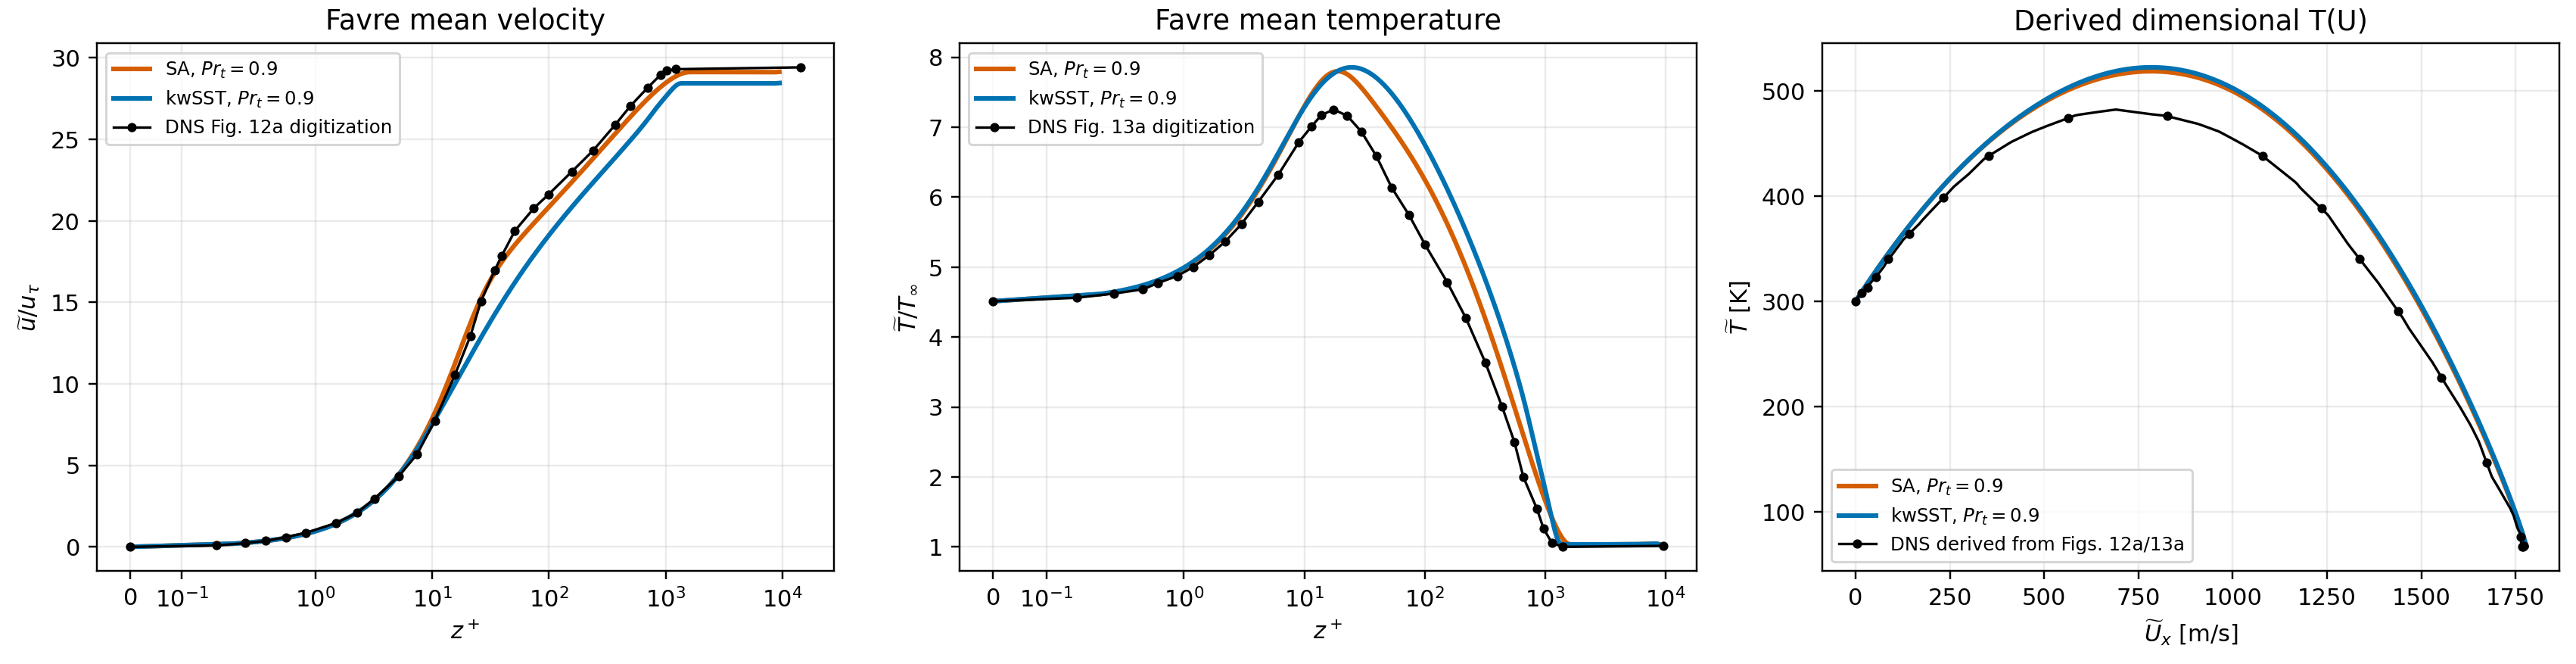
\includegraphics[width=\linewidth]{07_Error_Isolation_Results/Figures/Appendix/WR_BL_profile/Huang_BL2_profiles.png}
    \caption[Huang M11Tw020 at BL2: wall-resolved boundary layer profiles]{Wall-resolved Spalart--Allmaras and \(k\)--\(\omega\) SST profiles for M11Tw020 at station BL2 and \(Pr_t=0.9\), compared with DNS data digitized from Huang et al.~\cite[Figures~12(a) and 13(a)]{huang2020simulation}. Left: Favre-averaged velocity \(\widetilde{u}/u_\tau\) versus \(z^+\). Middle: temperature \(\widetilde{T}/T_\infty\) versus \(z^+\) at the matched \(Re_{\delta2}\) = 3419 station. Right: the corresponding dimensional temperature--velocity relation.}
    \label{fig:app:zpg:profiles:Huang-BL2}
\end{figure}

\end{landscape}
